% Should be ~2 pages 

% TODO: [Comment] It's easy to make a lists! Harder to produce a coherent picture of how pieces fit together. Tru to give treader details s/he needs to know when they become impatient for understanding or put them in background sections, -> e.g. do we need to know about kickstarter to understand that the fipy is a microcontroller that will collect measurements and send them to cloud?
\section{Components}  
\begin{itemize}
  
  \item \textbf{FiPy:} a microcontroller (not to be confused with the python package of the same name) that gives access to all major LPWAN technologies, originally funded through kickstarter.\cite{fipy-kickstarter} FiPy is developed by the IoT company PyCom\cite{pycom} and equipped with an expansion board to enable integration with other components via GPIO pinouts, as well as an LTE-antenna to enable LTE CAT M1 or NB1.\cite{fipy-docs} The board is programmed via the MicroPython programming language (an implementation of Python 3) which is written in C and optimized to run on a microcontroller.\cite{micropython-github}


  \item 
    \parbox[t]{\dimexpr\textwidth-\leftmargin}{%
    \vspace{-2.5mm}
    \begin{wrapfigure}{r}{0.4\textwidth}
      \centering
      \vspace{-\baselineskip}
      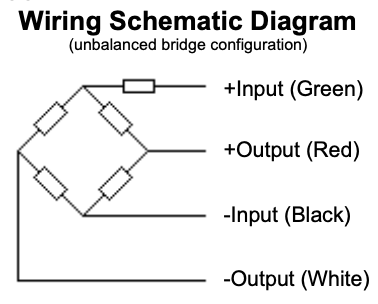
\includegraphics[scale=0.5]{load-cell-wiring.png}
      \caption{Wiring schematic\cite{load-cell-manual}}
      \label{fig:wiring}
    \end{wrapfigure}
    \textbf{Tedea Huntleigh - Model 1022:} a single point load cell ideally suited for low cost weighing platforms. This specific model has the capacity of ~30 kg.\cite{load-cell-manual} It is a type of strain gauge load cell which converts the physical load it's exposed to to electrical signals. When a weight is applied, the metal deforms slightly, which changes the internal electrical resistance and therefore affects the output of the voltage.\cite{strain-gauge} To utilize the load cell, the four wires need to be hooked up as according to figure \ref{fig:wiring}.
    }


  \item 
    \parbox[t]{\dimexpr\textwidth-\leftmargin}{%
    \vspace{-2.5mm}
    \begin{wrapfigure}{l}{0.4\textwidth}
      \centering
      \vspace{-\baselineskip}
      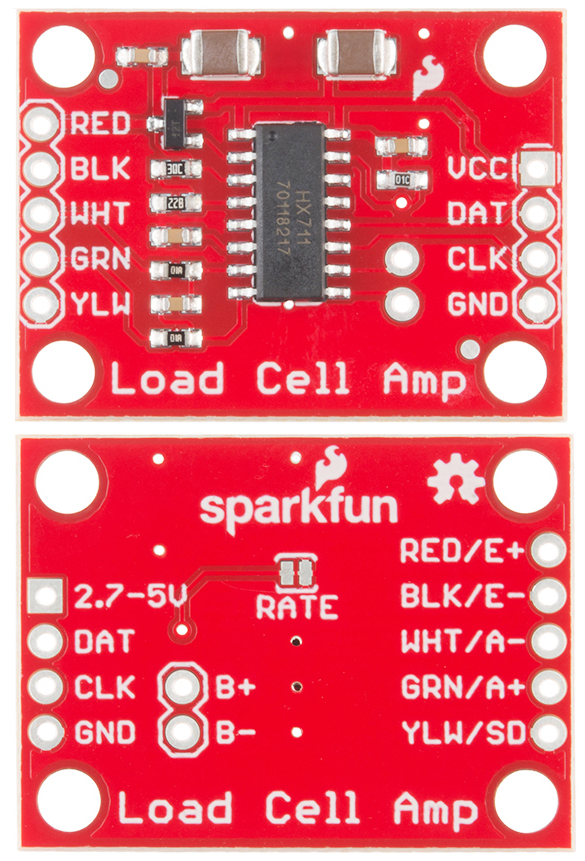
\includegraphics[scale=0.1]{hx711.png}
      \caption{HX711\cite{hx711-shop}}
      \label{fig:hx711}
    \end{wrapfigure}
    \textbf{HX711:} a breakout board that amplifies the signal from a load cell so that the data can be read more easily. Since the load cell outputs an analog signal in the form of mV/V, a conversion to a digital format is needed. It's important to note the industry standard of the wire coloring in load cells is not definitive.\cite{load-cell-wiring-standard} If the wires are from the model 1022 are connected in the sockets as figure \ref{fig:hx711} suggests, the load cell will not work correctly. According to figure \ref{fig:hx711} and figure \ref{fig:wiring} we can see that the green and red wire needs to switch places, because of E+ corresponding to Input+ and A+ corresponding to Output+.
    }

\end{itemize}


\section{Applications \& Services}
\lipsum[2]
% TODO: Describe PyBytes